\RequirePackage[T1]{fontenc}
\documentclass[conference]{IEEEtran}
\usepackage{amsmath,amssymb,booktabs,graphicx,url,capt-of,longtable,balance}
\usepackage[hidelinks]{hyperref}
\setcounter{topnumber}{3}
\setcounter{dbltopnumber}{3}
\renewcommand{\topfraction}{0.92}
\renewcommand{\dbltopfraction}{0.92}
\renewcommand{\textfraction}{0.06}
\renewcommand{\floatpagefraction}{0.8}
\renewcommand{\dblfloatpagefraction}{0.8}
\graphicspath{{../results/controlled_experiment/analysis_v1/}{../results/connectivity_experiment/analysis_v2/}}
% Generated from validated statistics; do not edit numbers manually.
\newcommand{\LegacySuccess}{21.4}
\newcommand{\RewardOnlySuccess}{100.0}
\newcommand{\FixedSuccess}{99.7}
\newcommand{\TerminationSuccess}{0.0}
\newcommand{\PrimaryGain}{78.3}
\newcommand{\CILower}{66.2}
\newcommand{\CIUpper}{89.5}
\newcommand{\RewardOnlyLongSuccess}{100.0}
\newcommand{\FixedLongSuccess}{36.1}
\newcommand{\FixedLongSD}{12.6}
\newcommand{\FixedFeasible}{97.8}
\newcommand{\PDSuccess}{100.0}
\newcommand{\PDLongSuccess}{100.0}
\newcommand{\LegacyTime}{141.2}
\newcommand{\RewardOnlyTime}{50.2}
\newcommand{\FixedTime}{36.5}
\newcommand{\PDTime}{28.6}
\newcommand{\FixedMinusPDTime}{7.9}
\newcommand{\TrainingMinutes}{9.4}

\newcommand{\ind}{\mathbb{1}}
% Generated from frozen connectivity statistics. Do not edit numbers manually.
\newcommand{\FullStd}{96.6}
\newcommand{\ArrivalStd}{96.9}
\newcommand{\SuccessDeltaStd}{-0.3}
\newcommand{\SuccessLowStd}{-2.6}
\newcommand{\SuccessHighStd}{2.0}
\newcommand{\CostChangeStd}{-24.5}
\newcommand{\DelayChangeStd}{186.7}
\newcommand{\HandoverChangeStd}{-95.5}
\newcommand{\FullFailuresStd}{34}
\newcommand{\CommonStd}{945}
\newcommand{\FullLong}{89.7}
\newcommand{\ArrivalLong}{86.3}
\newcommand{\SuccessDeltaLong}{3.4}
\newcommand{\SuccessLowLong}{-1.0}
\newcommand{\SuccessHighLong}{8.1}
\newcommand{\CostChangeLong}{-14.7}
\newcommand{\DelayChangeLong}{261.1}
\newcommand{\HandoverChangeLong}{-92.8}
\newcommand{\FullFailuresLong}{103}
\newcommand{\CommonLong}{802}

\title{Reward Repair and Connectivity Constraints for Cellular UAVs:\\Two Studies on a Barcelona Radio Map}
\author{\IEEEauthorblockN{Guillem Moreno Garcia and Evgenii Vinogradov}
\IEEEauthorblockA{Universitat Polit\`ecnica de Catalunya, Barcelona, Spain\\Research draft, 12 September 2026}}
\begin{document}
\maketitle
\begin{abstract}
A cellular UAV must reach its destination while satisfying communication
requirements. We investigate a master's thesis reward formulation through two
separately frozen reimplementation studies on a received Barcelona ray tracing
map. Study I crosses reward replacement and arrival termination across four
PPO treatments and five training seeds. Standard arrival rises from
\LegacySuccess\% for the legacy reward to \RewardOnlySuccess\% for reward
replacement alone; termination alone achieves \TerminationSuccess\%.
The combined change achieves \FixedSuccess\% standard arrival but only
\FixedLongSuccess\% on longer routes. A subsequent audit shows why this is
insufficient: only 92.2\% of the reward only standard flights avoid every
sampled RSS outage. Study II enforces minimum RSS and bounded queue occupancy,
restores delay, interference and handover costs, and adds explicit resource
choices and a shared prospective safety filter. Five seeds per arm yield
\FullStd\% standard and \FullLong\% longer joint success with full radio cost,
versus \ArrivalStd\% and \ArrivalLong\% without it. On paired successful
standard flights, weighted radio cost falls 24.5\%, but delay rises 186.7\%.
A deterministic radio selection reference achieves 98.0\% and 92.5\% joint
success. The evidence supports a reward and endpoint repair within the declared
surrogate, with retained negative findings and explicit thesis page comparisons;
it establishes neither a PPO advantage nor reproduction of the original simulator.
\end{abstract}
\begin{IEEEkeywords}
Cellular UAV, reward shaping, connectivity constraints, handover, resource
allocation, reinforcement learning, reproducibility.
\end{IEEEkeywords}

\section{Introduction}
A 2026 master's thesis uses a Barcelona ray tracing environment for joint UAV
trajectory and handover control~\cite[pp.~6--7, Sec.~3.1]{thesis}. Its objective
combines delay, interference and handovers~\cite[p.~10, Eq.~(11)]{thesis}, with
minimum RSS and bounded queue constraints~\cite[p.~11, Eq.~(12), C2 and C4]{thesis}.
The reward gives a fixed bonus whenever distance decreases
\cite[p.~12, Eqs.~(13)--(14); p.~15, Table~3]{thesis}, while training continues
after arrival to encourage braking~\cite[p.~12, Sec.~5.2]{thesis}. The thesis
reports wandering and prioritization of connectivity over destination completion
\cite[p.~19, Sec.~7.2; p.~21, Sec.~8]{thesis}. Its listed observation omits
velocity despite acceleration control~\cite[p.~12, Sec.~5.2; p.~9, Eq.~(2)]{thesis}.
These are reasons to audit the formulation; they do not identify the exact
behavior of unavailable source code. All thesis locators here use printed
pages; add two to obtain the PDF viewer page.

Cellular control couples flight, association and resources. Related work
jointly studies cargo UAV paths and association~\cite{cherif}; hybrid control
\cite{hybrid}, invalid action masking~\cite{masking}, and potential based
shaping~\cite{shaping} provide established tools. We contribute a controlled
empirical diagnosis with reproducible artifacts, rather than a new algorithm
or shaping theorem.

The two studies answer different questions. Study I isolates replacement of
the written reward and termination on safe arrival within one shared surrogate.
Its positive arrival result is then audited against the full communication
task. Study II compares an arrival objective with the same objective plus all
three communication costs under strict sampled RSS and queue constraints.
Its controller and training range also change, so comparisons between studies
are descriptive; only within study contrasts isolate their declared factors.

Both studies retain five training seeds per learned treatment, fresh test
routes, deterministic references, unsuccessful designs and all reported
failure outcomes. The original simulator and trained policies remain unavailable.
We therefore make no claim of improvement over the thesis's actual controller.
The received private map has matching metadata, not verified experiment version
identity. Detailed appendices distinguish original definitions, shared
reimplementation choices, treatment factors, and the subsequent connectivity
repair. Favorable aggregate communication cost never replaces the primary
mission outcome or the individual radio components.

\section{Data and Initial Shared Surrogate}
\label{sec:shared}
The following model defines Study I and the common physical assumptions retained
in Study II. Its permissive connectivity endpoint is superseded in
Study II, as described in Section~\ref{sec:joint}.

\subsection{Received Radio Map}
The file \texttt{Barcelona\_dataset\_January.h5} contains an
\(133\times5000\times3500\) signed 8 bit RSS array, station identities and
coordinates, operator membership, and transmit powers. Its metadata gives
2.1 GHz, 100 m altitude, and nominal 1 m grid resolution. The file size is
2,327,593,160 bytes. We use the 87 station operator corresponding to the thesis's
first operator~\cite[p.~14, Sec.~6.1]{thesis}. The station counts, frequency,
height, and dimensions match the description~\cite[p.~6, Sec.~3.1.1;
p.~7, Table~2]{thesis}, but exact experiment version identity is not established.

The original stored coordinate vectors span 0--5000 m with 5000 samples and
0--3500 m with 3500 samples. Their spacings are approximately 1.00020004 m and
1.00028580 m. Nearest neighbor lookup uses these vectors; all training and
evaluation use native resolution. Values are promoted to floating point before
radio arithmetic. The untouched source checksum and schema are retained.

A full scan finds that 27.77245\% of all link entries equal $-128$, while the
other entries range from $-110$ to $-25$ dBm. We provisionally interpret $-128$
as an absent usable path and assign it zero received power. The generator's
sentinel and quantization conventions still require confirmation. For the
selected operator, every grid position has at least 38 stations above
$-96$ dBm, and the strongest RSS ranges from $-51$ to $-25$ dBm. Thus the stored
map has no inevitable geographic coverage hole under this RSS threshold.
This observation does not guarantee a permissible handover or adequate SINR.

\subsection{Motion, Mission, and Observations}
The thesis writes scalar speed and a selected direction in its position update
\cite[p.~9, Sec.~3.2, Eq.~(2)]{thesis}. Our shared benchmark instead preserves
an inertial velocity vector at constant altitude. With velocity projection,
\begin{align}
\mathbf v_{t+1}&=\Pi_{\|\mathbf v\|\leq v_{\max}}
 (\mathbf v_t+\mathbf a_t\Delta t),\\
\mathbf p_{t+1}&=\mathbf p_t+
 \tfrac12(\mathbf v_t+\mathbf v_{t+1})\Delta t.
\end{align}
The policy supplies radial and lateral acceleration components in a frame
aligned with the current destination bearing. Their norm is limited to
5 m/s$^2$, and speed is limited to 25 m/s. This continuous action interface
replaces the five acceleration bins and eight headings
\cite[p.~12, Sec.~5.2; p.~15, Table~3]{thesis}. The thesis uses a 100 m/s
penalty threshold~\cite[p.~15, Table~3]{thesis}; ours is a hard 25 m/s cap.
The step is 1 s and the deadline is 200 s. The source gives 1 ms in prose
\cite[p.~14, Sec.~6.1]{thesis} and 0.1 s in Table~3
\cite[p.~15]{thesis}; we explicitly choose a new time discretization.

Safe arrival is the common event
\begin{equation}
\mathcal G_t=\{\|\mathbf p_t-\mathbf g\|\leq10\ \mathrm m,
                  \ \|\mathbf v_t\|\leq2\ \mathrm{m/s}\}.
\end{equation}
The 10 m position tolerance is retained from Table~3~\cite[p.~15]{thesis};
the numerical 2 m/s terminal speed test is our addition to the stated stopping
intention~\cite[p.~9, Sec.~3.2]{thesis}. A boundary crossing, battery exhaustion,
or five consecutive RSS outage samples ends a failure. The thesis explicitly
terminates on energy exhaustion and penalizes boundary, RSS, and speed
violations~\cite[p.~12, Sec.~5.2, Eq.~(14)]{thesis}; our boundary and repeated
outage terminations are additional rules. Speed is constrained directly.
Building geometry supports propagation in the thesis~\cite[p.~6, Sec.~3.1.1]{thesis}.
Our received RSS array does not provide a collision model, and obstacle safety
is outside the evaluated model; we do not assume the original code enforced it.

Every treatment receives the same 42 dimensional observation: position;
destination bearing and distance; radial, lateral, and total velocity;
remaining time encoded by elapsed time; energy; buffer; prior arrival flag;
resource and load phases; network decision phase; serving SINR; outage count;
and candidate RSS, relative positions, identities, and masks. This replaces
the listed six component vector of position, serving station, resource group,
energy, and buffer~\cite[p.~12, Sec.~5.2]{thesis}. Observation repair is shared,
and its independent effect is not estimated.

\subsection{Association and Communication Proxies}
A categorical policy selects stay or one of the four strongest candidate
stations. A request is admissible when candidate RSS exceeds both $-96$ dBm
and serving RSS plus 3 dB. Network actions occur every five seconds, with an
additional opportunity on an observed serving RSS outage. This emergency rule
was introduced during validation, before training, when a periodic decision
could otherwise arrive after the outage failure deadline. We do not implement
or claim a complete 3GPP time to trigger procedure. Masking follows the standard
practice of excluding invalid categorical actions~\cite{masking}.
The inequality follows the thesis's A3 equation~\cite[p.~9, Eq.~(3)]{thesis},
with the numerical offset from Table~3~\cite[p.~15]{thesis}; the five action
candidates and decision interval are our choices. The source greedy controller
uses viability counters~\cite[pp.~13--14, Sec.~5.4]{thesis}, which we do not copy.

There are twelve resource groups and six occupied background groups per
station in a fixed spatial pattern. A shared first available allocation rule
chooses the resource group; resource allocation is not learned. Scenario phase
rotates group labels globally and does not supply independent traffic dynamics.
The source permits learned RBG requests~\cite[p.~9, Sec.~3.3.1;
p.~12, Sec.~5.2]{thesis} and describes random occupancy of at least half the
groups~\cite[p.~14, Sec.~6.1]{thesis}; both differ from our shared allocator.
Since the source RSS is a downlink budget~\cite[p.~7, Eq.~(1)]{thesis}, station powers
are aggregated as a downlink interference proxy:
\begin{equation}
P_k=10^{(\mathrm{RSS}_k-30)/10},\quad
\mathrm{SINR}=\frac{P_s}{N+\sum_{k\ne s}o_kP_k}.
\end{equation}
Here powers are in watts, $o_k$ indicates background occupancy of the selected
group, and noise including the noise figure is $-103.41$ dBm. The ideal service
rate is $1.44\cdot10^6\log_2(1+\mathrm{SINR})$ bit/s. It is neither measured
throughput nor a validated uplink interference model.
This replaces the printed bandwidth-plus-logarithm rate, SNR in dB, and sum of
RSS values labeled uplink interference~\cite[p.~10, Eqs.~(7)--(9)]{thesis}.
It changes the interference model as well as correcting power arithmetic;
we cannot establish whether the original code used the printed expressions.

Deterministic offered traffic is 200 kbit/s, buffer capacity is 1.28 Mbit, and a
handover adds 4800 bits. The control overhead and nominal buffer capacity follow
Table~3~\cite[p.~15]{thesis}, interpreting KB as decimal kilobytes.
Deterministic traffic replaces the Poisson formulation
\cite[pp.~9--10, Eqs.~(5)--(6)]{thesis}; the thesis also gives different data
packet sizes in prose and table~\cite[pp.~14--15, Sec.~6.1, Table~3]{thesis}.
The backlog/service delay retains the ratio in Eq.~(4)~\cite[p.~9]{thesis},
but we explicitly use postservice backlog and censor at 200 s.
Energy is the integral
of $100+0.4\|\mathbf v\|^2$ watts against a 100 kJ budget. This explicit proxy
replaces the mass, efficiency, lift-to-drag and electronics expression
\cite[p.~10, Eq.~(10)]{thesis} and the capacity labeled 1000 kW
\cite[p.~15, Table~3]{thesis}. It does not claim a calibrated rotorcraft model.
Table~\ref{tab:changes}
summarizes the main departures from the source description.

\begin{table}[t]
\caption{Shared reimplementation choices, held fixed across treatments}
\label{tab:changes}\centering\footnotesize
\begin{tabular}{@{}p{.29\columnwidth}p{.64\columnwidth}@{}}
\toprule
Aspect & Declared benchmark choice\\\midrule
Observations & Goal and velocity observed; 42 dimensions\\
Motion & Continuous acceleration, 1 s steps, 25 m/s cap\\
Network & Stay plus four candidates; masks; outage requests\\
Resources & Common deterministic first available allocator\\
Interference & Linear downlink cochannel power proxy\\
Traffic and energy & Deterministic traffic; explicit energy proxy\\
Source equivalence & Original code and checkpoints unavailable\\\bottomrule
\end{tabular}
\end{table}

\section{Study I: Reward and Arrival Termination}
\label{sec:study1}
\subsection{Why the Binary Approach Bonus Is Suspect}
Let $d_t$ be destination distance, $D_t$ the declared delay proxy, $I_t$ the
linear interference proxy, and $h_t$ a handover indicator. The legacy reward
treatment implements the structure in Eqs.~(13)--(14)
\cite[p.~12]{thesis}, with the equal-policy weights, scales, and bonus in
Table~3~\cite[p.~15]{thesis}:
\begin{align}
r_t^L={}&\frac{.35}{1+10D_t}+\frac{.30}{1+10^5I_t}
       +\frac{.35}{1+100h_t} \nonumber\\
       &+12\ind[d_{t+1}<d_t]-10O_t-10B_t,
\end{align}
where $O_t$ and $B_t$ mark RSS outage and a boundary crossing. Energy exhaustion
overrides the reward with $-10$. The shared speed constraint replaces a soft
speed penalty. The interference input is corrected to watts for all treatments;
thus this is an ablation of the written incentive, not literal replication of
potentially erroneous source equations.

The approach term depends on the sign of progress but not its magnitude. A
controller can receive the same bonus for very slow progress as for efficient
flight. A retreat carries no matching distance cost, permitting positive
approach bonuses on a closed excursion outside the destination region.
Moreover, stopping the episode without a compensating mission objective can
remove future positive reward and reinforce avoidance of completion. Similar
failures motivate potential based shaping~\cite{shaping}.

\subsection{Mission Reward and Terminal Potential}
Define the potential, with $L=100$ m,
\begin{equation}
\Phi(s)=-\frac{d+\|\mathbf v\|^2/(2a_{\max})}{L}.
\end{equation}
The speed term is a stopping distance scale. The replacement reward is
\begin{align}
r_t^M={}&20A_t-20F_t-0.05-0.05c_t \nonumber\\
        &+\gamma\Phi(s_{t+1})-\Phi(s_t),
\end{align}
where $A_t$ marks first safe arrival, $F_t$ a terminal failure before any safe
arrival, and $c_t=\min(D_t,1)+O_t+h_t$. The prior arrival flag is observed, and
the success bonus is paid only once even if training continues afterward.
Set the potential to zero at every terminal, including the deadline. For any
episode ending at $T$, the shaping contribution satisfies
\begin{equation}
\sum_{t=0}^{T-1}\gamma^t
 [\gamma\Phi(s_{t+1})-\Phi(s_t)]=-\Phi(s_0).
\end{equation}
Consequently, within each fixed terminal formulation, shaping preserves the
discounted base objective~\cite{shaping}. This identity is checked numerically.
It does not imply that the finite weighted base reward certifies every physical
constraint or guarantees successful learning.
The identity concerns raw rewards. Running normalization and clipping in PPO
can change the effective update objective; this experiment tests the declared
learning recipe without isolating those interactions.

\begin{table}[t]
\caption{Factorial training treatments}
\label{tab:arms}\centering\footnotesize
\begin{tabular}{lll}\toprule
Label & Reward & Terminate on arrival\\\midrule
Legacy & $r^L$ & No\\
Termination only & $r^L$ & Yes\\
Reward only & $r^M$ & No\\
Both & $r^M$ & Yes\\\bottomrule
\end{tabular}
\end{table}

\begin{figure}[!t]
\centering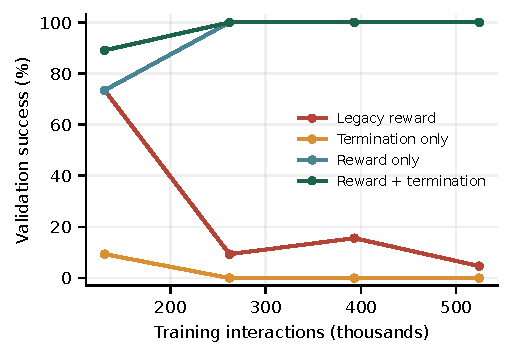
\includegraphics[width=.98\columnwidth]{pilot_learning.pdf}
\caption{Pilot seed 42 on 64 validation routes. Curves are used to document
development and budget choice, not to substitute for the frozen test comparison.}
\label{fig:pilot}
\end{figure}

\subsection{Common PPO Implementation}
All arms use proximal policy optimization~\cite{ppo} with separate actor and
critic networks, each containing two 64 unit tanh layers. The actor has a
Gaussian motion head and a masked categorical association head. Motion samples
are transformed through tanh and the acceleration norm limit; likelihood ratios
are consistently computed in latent action space. The entropy regularizer sums
latent Gaussian and masked categorical entropy.

Training uses 64 parallel lanes, 128 step rollouts, four epochs per rollout,
512 sample minibatches, Adam learning rate $3\cdot10^{-4}$, clip 0.2,
$\gamma=0.99$, GAE parameter 0.95, entropy coefficient 0.005, value coefficient
0.5, and gradient norm limit 0.5. Rewards are divided by a running standard
deviation of discounted returns without subtracting a mean, and clipped to
$[-10,10]$, consistently across arms. Finite horizon terminals are not
bootstrapped. No pretrained model, demonstrations, or imitation loss is used.
The thesis uses Stable Baselines~\cite[p.~13, Sec.~5.3]{thesis}; our PPO is a
new native implementation. Table~\ref{tab:ppocomparison} contrasts every
reported source setting with ours~\cite[p.~16, Table~4]{thesis}.
For example, learning rate increases from $3\cdot10^{-5}$ to $3\cdot10^{-4}$,
entropy weight decreases from 0.01 to 0.005, and the source's 0.03 target KL
is replaced by diagnostic KL logging without an early stopping threshold.

\begin{table*}[t]
\caption{Frozen results: percentages are mean $\pm$ standard deviation over five training seeds. Standard routes are 200--1000 m; longer routes are 1000--1800 m. Each learned policy evaluates 200 routes per split.}
\label{tab:results}\centering\footnotesize
\begin{tabular}{lcccccc}\toprule
 & \multicolumn{2}{c}{Mission success (\%)} & \multicolumn{2}{c}{Recorded feasible success (\%)} & \multicolumn{2}{c}{Successful episodes}\\
Treatment & Standard & Longer & Standard & Longer & Standard & Longer\\\midrule
Legacy & $21.4\pm14.3$ & $0.0\pm0.0$ & $20.8\pm13.9$ & $0.0\pm0.0$ & 214/1000 & 0/1000 \\
Termination only & $0.0\pm0.0$ & $0.0\pm0.0$ & $0.0\pm0.0$ & $0.0\pm0.0$ & 0/1000 & 0/1000 \\
Reward only & $100.0\pm0.0$ & $100.0\pm0.0$ & $98.7\pm1.4$ & $96.0\pm1.1$ & 1000/1000 & 1000/1000 \\
Both & $99.7\pm0.7$ & $36.1\pm12.6$ & $97.8\pm0.8$ & $35.2\pm12.6$ & 997/1000 & 361/1000 \\
Deterministic reference & 100.0 & 100.0 & 97.0 & 95.5 & 200/200 & 200/200 \\
\bottomrule\end{tabular}
\end{table*}


\begin{figure*}[!t]
\centering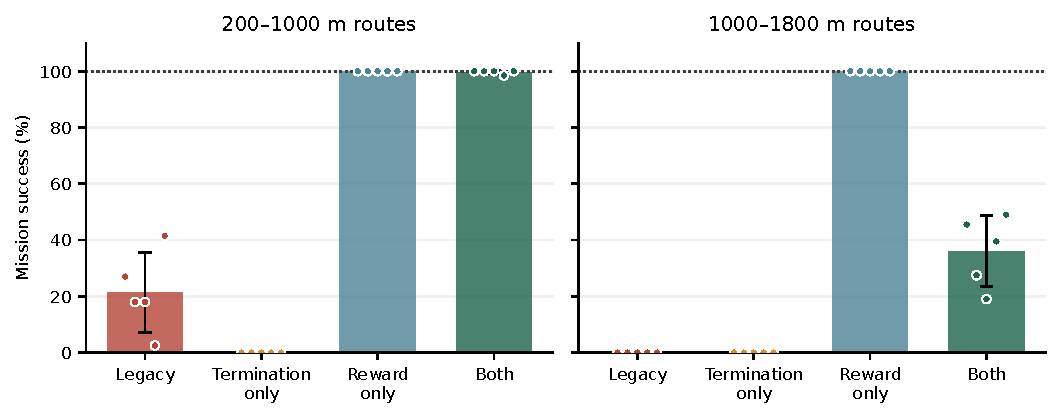
\includegraphics[width=.97\textwidth]{success_comparison.pdf}
\caption{Study I arrival success under its permissive connectivity rules. Each dot is one training seed, bars show
the mean, and error bars show seed standard deviation. There are 200 shared
routes per split and five seeds per learned treatment. The dotted line is the
deterministic reference. No test outcome was used to tune the frozen policies.}
\label{fig:arrival_success}
\end{figure*}

\subsection{Validation, Freeze, and Held Out Routes}
Training uses 4096 routes sampled with lengths 200--1000 m, with 64 separate
validation routes. The final standard set contains 200 new routes of the same
length range. A second set contains 200 routes of length 1000--1800 m. These
are unseen coordinate pairs in the same city, not independent cities or held
out geographic regions. Starts and destinations stay inside documented map
margins. All coordinates, seeds, and background phases are saved.
The original tuning and comparison sections do not specify three independent
training, validation, and test route sets~\cite[pp.~15--16, Secs.~6.2--6.3]{thesis}.
This is a limit of the written protocol, not proof that its unavailable code
lacked such a separation.

Six pilots, using seeds 41 and 42, established learning behavior and the
524,288 interaction budget. All final arms use seeds 1101--1105 and exactly
that budget, totaling 10,485,760 interactions. Source hashes and configuration
were frozen before trained policy test evaluation. The initial feasibility
inspection used separate exploratory route sets, which were retired before
training; final route seeds are 42012 and 42013. Final checkpoints are evaluated
without early stopping or test based selection. Each lane follows the same
ordered training scenario stream across treatments, although successful
termination changes how many episodes fit in an equal interaction budget.

The evaluated continuous action is the Gaussian mean after transformation, and
the network action is the masked categorical mode. Every policy's evaluation
stops at first safe arrival, independently of its training termination rule.
Thus the continuing training treatment is still evaluated as a finite mission.

\subsection{Metrics, Reference, and Uncertainty}
Study I arrival success is primary. Its historical recorded feasible success additionally requires
no packet overflow and an RSS outage fraction at most 5\%. This limited
feasibility label does not imply obstacle or airframe certification. Failure
counts and final distances are retained. Time, path, energy proxy, delay,
interference, SINR, and handovers are reported conditional on success with
their sample counts, avoiding aggregation of failed flights into radio gains.

The deterministic reference points its desired velocity toward the goal, uses
a braking schedule based on stopping distance, and requests the strongest
admissible station. It shares every environmental constraint and resource rule.
It establishes that the tested missions are attainable and provides a practical
nonlearning comparison; it is not asserted to be globally optimal.

We show all five seed outcomes and standard deviations. The primary contrast
is both changes minus legacy success on standard routes. A 10,000 draw crossed
bootstrap resamples the five seed identities and 200 route identities, using
the same sampled identities for both arms. This preserves pairing and avoids
counting 1000 episodes as 1000 independent training runs. Other factorial and
longer route contrasts are secondary. Interval reporting follows the broader
need to expose uncertainty in few run RL evaluations~\cite{statistics}.
Five seeds still provide limited resolution and uncertain tail behavior.

The prespecified practical gate for a positive repair finding requires at least
90\% mean standard mission success, at least 90\% recorded feasible success,
and a positive lower 95\% bootstrap bound for the primary contrast. It is a
reporting gate rather than a claim of statistical or deployment certification.

\begin{figure*}[!t]
\centering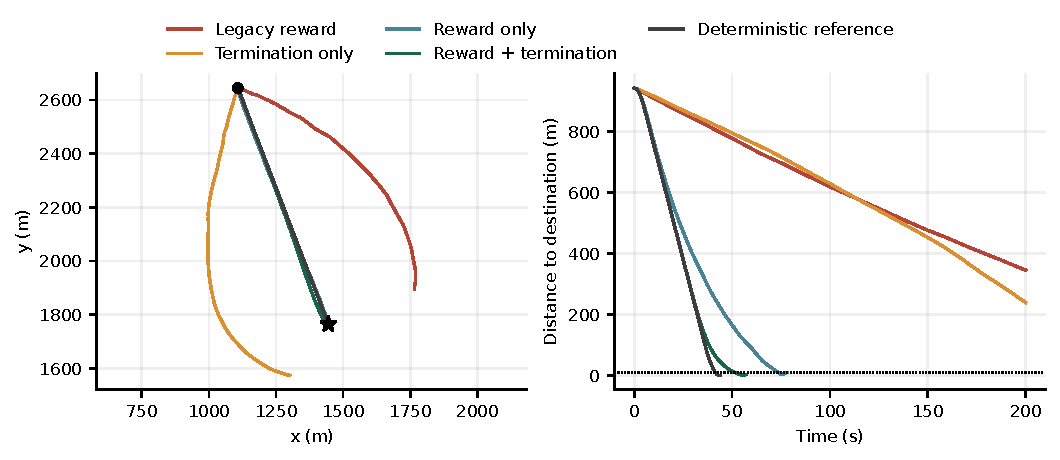
\includegraphics[width=.97\textwidth]{example_trajectory.pdf}
\caption{First standard test route and first declared training seed. The black
circle and star denote start and destination. All learned treatments and the
deterministic reference share the scenario. The dotted distance line marks
10 m; low speed is also required for success.}
\label{fig:trajectory}
\end{figure*}

\begin{table*}[t]
\caption{Standard route metrics conditional on mission success, pooled across the five seeds. The deterministic reference has one run on 200 routes. Different successful subsets prevent unqualified secondary dominance claims. Energy, delay, and interference are the declared proxies.}
\label{tab:metrics}\centering\footnotesize
\begin{tabular}{lrrrrrrrr}\toprule
Treatment & $n$ & Time (s) & Energy (kJ) & Handovers & SINR (dB) & Delay (s) & Outage (s) & Interf. ($\mu$W)\\\midrule
Legacy & 214 & 141.25 & 14.80 & 8.83 & -6.34 & 0.88 & 0.07 & 0.70 \\
Termination only & 0 & n/a & n/a & n/a & n/a & n/a & n/a & n/a \\
Reward only & 1000 & 50.23 & 8.29 & 3.96 & -7.91 & 2.58 & 0.09 & 0.74 \\
Both & 997 & 36.52 & 8.17 & 2.99 & -8.13 & 2.83 & 0.09 & 0.74 \\
Deterministic reference & 200 & 28.62 & 7.99 & 2.38 & -8.51 & 3.45 & 0.09 & 0.74 \\
\bottomrule\end{tabular}
\end{table*}


\subsection{Completion and Factorial Effects}
Table~\ref{tab:results} and Fig.~\ref{fig:arrival_success} present the full frozen
comparison. Reward replacement alone achieves \RewardOnlySuccess\% standard
success compared with \LegacySuccess\% for the legacy reward. The combined
change achieves \FixedSuccess\%, while termination alone achieves
\TerminationSuccess\%. The primary gain is \PrimaryGain\ percentage points,
with a paired bootstrap interval [\CILower, \CIUpper]. Recorded feasible
success for the combined change is \FixedFeasible\%, satisfying the practical
arrival gate. This gate did not require uninterrupted sampled connectivity.
These results identify the replacement reward as the essential tested
intervention; changing arrival termination alone does not resolve the failure.

The pilots also illustrate why longer training cannot automatically repair a
misaligned objective. In pilot seed 42, legacy validation success initially
rises to 73.4\% and then falls to 4.7\% by the final budget. Reward replacement
reaches 100\% by approximately 262,144 interactions and retains it through
the pilot's final checkpoint. Figure~\ref{fig:pilot} is explicitly exploratory
validation evidence from one pilot, not a confidence interval over final seeds.

\subsection{Longer Routes and the Role of Termination}
Reward replacement with continuing training reaches \RewardOnlyLongSuccess\%
success on longer routes. The combined treatment reaches
\FixedLongSuccess\% with seed standard deviation \FixedLongSD\ percentage
points. Thus the treatment that provides efficient completion within the
training range does not necessarily generalize best to longer flights.
Training termination changes episode exposure and visitation distribution even
under equal interaction budgets, but the experiment does not isolate the
mechanism causing this extrapolation difference. The longer route weakness is
retained rather than removed by further test driven tuning.

Figure~\ref{fig:trajectory} shows the first predefined standard test route for
seed 1101, selected by index rather than performance. Its trajectories and
distance traces illustrate the different learned behavior, while the aggregate
tables remain the basis for the conclusions. Proximity by itself is insufficient:
the evaluated success criterion also requires low speed.

\subsection{Efficiency and the Deterministic Reference}
The deterministic reference achieves \PDSuccess\% standard and
\PDLongSuccess\% longer route success. Among successful standard missions,
mean flight times are \LegacyTime\ s for legacy, \RewardOnlyTime\ s for
reward only, \FixedTime\ s for both changes, and \PDTime\ s for the reference.
Because the successful subsets differ, these means alone are not paired
efficiency comparisons. On matched successful standard routes, the combined
policy takes \FixedMinusPDTime\ s more time than the reference on average.
The evidence establishes repair of a learned objective, not an advantage over
the deterministic controller.

Table~\ref{tab:metrics} reports success conditional secondary metrics with
sample counts. The radio summaries are downlink proxies and the energy measure
is uncalibrated. A controller with lower interference or delay on a subset of
completed short routes is not ranked above a controller that completes the
whole route set. Raw per episode records permit matched subset analysis without
concealing failures or mixing physical units.
The original results emphasize SNR, outage, interference, remaining energy,
and handover count~\cite[pp.~16--20, Sec.~7, Figs.~5--8]{thesis}.
Our success rate, terminal speed and distance checks, success conditional
reporting, and paired seed uncertainty are additional evaluation choices.

\section{Connectivity Requirements and the Study I Audit}
\label{sec:audit}
\subsection{Which Communication Requirements Apply?}
We use the thesis requirements, not a newly imposed application service level.
The RSS minimum is $-96$ dBm and the buffer is listed as 160 KB
\cite[p.~15, Table~3]{thesis}; we retain the explicit 1,280,000 bit interpretation.
The written C2 inequality allows equality and applies at every modeled time
\cite[p.~11, Eq.~(12)]{thesis}. Delay remains an optimized quantity, defined in
the source as queue divided by service rate~\cite[p.~9, Eq.~(4)]{thesis}.
Neither a two second packet deadline nor an empty queue arrival condition is
introduced. A successful arrival can therefore retain queued data; it must not
be described as completed data delivery.

The distinction between formulation and enforcement matters. The source reward
penalizes RSS violations~\cite[p.~12, Eq.~(14)]{thesis}, which does not establish
that its unavailable implementation guaranteed C2. Its direct data dump penalty
was removed during development~\cite[pp.~20--21, Sec.~7.3]{thesis}. We compare
verified written definitions with our executable rules, not inferred behavior
of missing original code.

\subsection{Why the Earlier Arrival Result Was Insufficient}
The original map audit found at least 38 operator 1 stations strictly above
$-96$ dBm at every grid location. The strongest station ranges from $-51$ to
$-25$ dBm. Consequently, an RSS coverage hole does not force a detour if any
suitable station could be selected. Actual association constraints and
interference still matter.

An exact replay of 4,400 Study I flights added service diagnostics without
changing their saved outcomes. In the earlier reward replacement's 1,000
standard evaluations, arrival was 100\%, but only 92.2\% had no sampled RSS
outage. Modeled capacity was below the 200 kbit/s offered rate for a mean
26.6\% of each flight, and 20.2\% arrived with a nonempty queue. A transient
capacity deficit is not itself disconnection because buffering can absorb it.
These measures expose what the old endpoint did and did not establish; they
are not a new confirmatory policy comparison.

\section{Study II: Strict Sampled Connectivity}
\label{sec:joint}
Study II retains the map, motion, radio arithmetic, traffic and energy
assumptions in Section~\ref{sec:shared}: 1 s steps, 5 m/s$^2$ acceleration,
25 m/s maximum speed, 200 s deadline, 100 kJ energy budget, 12 resource groups,
static half occupancy, and 200 kbit/s offered traffic. These remain explicit
surrogate choices. The changes below concern the mission endpoint, radio
objective and control architecture, not a recovered original simulator.

\subsection{Joint Success and Failure}
Let $d_t$ denote destination distance and $q_t$ the queue after the sampled
arrival/service update. Joint success requires arrival by the deadline with
$d_T\leq10$ m and $\|v_T\|\leq2$ m/s, together with
\begin{equation}
\mathrm{RSS}_{k_t}(p_t)\geq-96\ \mathrm{dBm},\quad
0\leq q_t\leq1{,}280{,}000\ \mathrm{bits},\quad\forall t.
\end{equation}
The 10 m tolerance follows the source table~\cite[p.~15, Table~3]{thesis}; the
numeric stopping tolerance is our explicit interpretation of stopping at the
destination~\cite[p.~9, Sec.~3.2]{thesis}. Map and energy conditions also apply.
A single sampled RSS violation or any buffer overflow ends a failed mission.
Failure takes precedence over simultaneous arrival. Initial RSS is checked;
queue clipping for storage cannot erase an overflow flag.

This enforces the constraints at modeled samples. It is not a guarantee
between the one second samples or within the queue update. No minimum SINR,
packet latency threshold, or final queue draining requirement is claimed.

\subsection{Actions, Residual Motion and Safety Filter}
The source includes BS and RBG actions~\cite[p.~12, Sec.~5.2]{thesis}. We expose
61 categorical options: stay, or five candidate station slots by 12 RBGs.
Candidates are serving plus the four strongest RSS stations. Masks reject
occupied groups and duplicated serving station slots. A new station must have
current RSS more than 3 dB above the serving RSS and meet the minimum, following
the source's A3 direction~\cite[p.~9, Eq.~(3); p.~15, Table~3]{thesis}.
Network decisions occur each modeled second, replacing the earlier surrogate's
five second interval. Resource changes within the same station are allowed and
counted separately from handovers. Handovers generate 4,800 control bits
\cite[p.~15, Table~3]{thesis}; switching interruption is not modeled.

The observation has 156 features covering geometry, velocity, time, queue,
energy, serving SINR, candidate RSS and positions, option capacities and masks.
Two Gaussian outputs define bounded residual acceleration commands. We project
a destination directed braking command onto the unit disk, add half of the
tanh transformed residual, and apply the shared acceleration projection. Both
learned arms use this prior; they do not learn basic flight entirely from
scratch. The source's fully discrete action and smaller state differ
\cite[p.~12, Sec.~5.2]{thesis}.

A shared safety filter predicts the proposed next position, RSS and queue. It
first tries another admissible station/resource pair for the same motion. If
none is feasible, it invokes the local motion/network search. If no candidate
repairs the step, the flight fails normally. The filter has prospective access
to the known map and is an explicit control component, not learned competence.
Interventions are recorded. It cannot establish global reachability.

\subsection{Restoring the Communication Objective}
Using source equal weights and scales~\cite[p.~15, Table~3]{thesis}, define
\begin{align}
C_t={}&0.35\frac{10D_t}{1+10D_t}
 +0.30\frac{10^5I_t}{1+10^5I_t}\nonumber\\
 &+0.35\frac{100H_t}{1+100H_t}.
\end{align}
Here $D_t$ is the backlog/service delay proxy in seconds, $I_t$ interference in
watts, and $H_t$ a handover indicator. These are one minus the source reciprocal
utilities~\cite[p.~12, Eq.~(13)]{thesis}, removing the positive reward for merely
remaining active while retaining all communication components. The earlier
replacement's flat delay penalty above one second is removed. The reciprocal
cost still saturates smoothly, which can favor substantial delay in exchange
for fewer handovers; it is not a latency guarantee.

Both learned arms use
\begin{equation}
\Phi_t=-\frac{d_t+\|v_t\|^2/(2a_{\max})}{100\ \mathrm{m}},
\end{equation}
with terminal potential zero. The base reward is $0.99\Phi_{t+1}-\Phi_t-0.05$,
plus 20 for joint success and minus 20 for terminal failure. The arrival arm
uses this base alone; the full arm subtracts $C_t$. Both have identical hard
failure rules and control interfaces. This is not a comparison to the original
trained thesis policy or a claim that a finite scalar reward proves optimal
lexicographic control.

\section{Study II Protocol and Results}
\label{sec:study2}
\subsection{Learning, Splits and Freeze}
PPO retains all optimizer, network width, rollout, normalization and discount
settings of Study I, with the categorical head expanded from five to 61 logits. Likelihoods refer to proposed residual
and network actions; projection and filtering are environment transformations.

Training has 4,096 routes of lengths 200--1800 m. Validation has 64 standard and
32 longer routes. Fresh tests contain 200 standard routes of 200--1000 m and
200 longer routes of 1000--1800 m. Exact route pairs do not overlap with the
earlier study or other v2 splits, but all use the same geographic map. Both
length ranges occur during training, so the longer set is not an extrapolation
test. The source does not document equivalent three way separation
\cite[pp.~15--16, Secs.~6.2--6.3]{thesis}.

Six development policies and unsuccessful local planning variants are retained
in Appendix~\ref{app:development}; their outcomes use validation routes only.
Final source, scenario and protocol hashes were frozen before test evaluation.
Each arm uses seeds 2101--2105 and 524,288 interactions, totaling 5,242,880 final
interactions across ten policies. Evaluation uses the final checkpoint and
deterministic actions; no test result selects a checkpoint or controller revision.

\subsection{References and Analysis}
Four deterministic references share the same filter and rules: nominal straight
flight with strongest RSS association (Goal RSS); the same nominal motion with
prospective station/resource cost minimization (Goal radio); a one step joint
search; and a three step joint search. Joint searches use nine initial motion
primitives: direction offsets and speed reductions of the braking reference.
They prioritize sampled feasibility and progress, then communication cost.
The three step search follows each initial choice with two predicted reference
steps. Both are local methods and may fail. The filter can alter nominally
straight motion, which is reflected in actual paths and intervention counts.

Primary reporting includes every mission and its failure reason. Secondary
communication comparisons use the intersection of successful paired routes;
intersection sizes and accumulated and average costs are retained. Paired
differences use 5,000 crossed bootstrap draws over seed identities and shared
route identities; deterministic comparisons resample routes only. Five training
seeds do not represent independent geographic or traffic realizations. The
prespecified strong joint improvement claim requires a positive lower interval
for completion improvement and a negative upper interval for accumulated
communication cost change. Individual components are reported regardless.

\begin{table}[!t]\centering
\caption{Joint success and successful standard mission cost. Learned rows aggregate five seeds on 200 routes; references use 200 routes.}
\label{tab:jointresults}
\begin{tabular}{lrrr}\toprule
Controller & Standard (\%) & Longer (\%) & $\sum C_t$\\\midrule
PPO arrival & 96.9 & 86.3 & 6.57\\
PPO full & 96.6 & 89.7 & 4.97\\
Goal RSS & 97.0 & 87.0 & 6.22\\
Goal radio & 98.0 & 92.5 & 3.23\\
Joint one step & 96.5 & 90.0 & 2.62\\
Joint three steps & 95.0 & 90.5 & 1.92\\
\bottomrule\end{tabular}
\end{table}

\begin{figure*}[!t]
\centering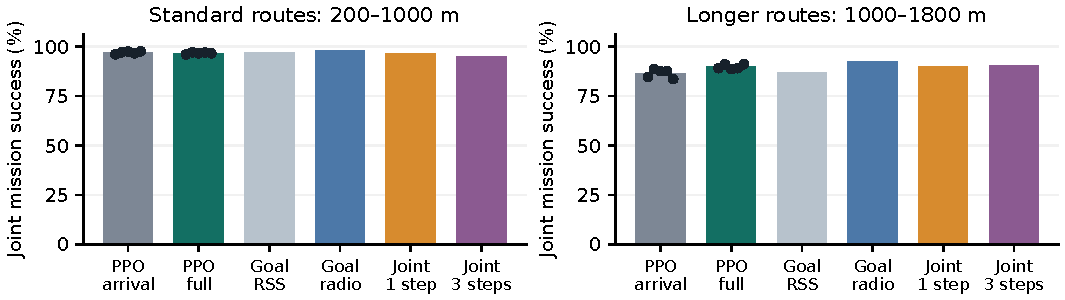
\includegraphics[width=.98\textwidth]{connectivity_success.pdf}
\caption{Strict sampled joint success on fresh routes. Dots show individual
training seeds for learned controllers. Deterministic controllers have one
evaluation per route, not five independent replications.}
\label{fig:joint_success}
\end{figure*}

\subsection{Strict Joint Completion}
Table~\ref{tab:jointresults} and Fig.~\ref{fig:joint_success} report the frozen results.
The full learned arm achieves \FullStd\% standard and \FullLong\% longer joint
success, compared with \ArrivalStd\% and \ArrivalLong\% for the arrival arm.
The paired standard completion difference is \SuccessDeltaStd\ percentage
points, with 95\% interval [\SuccessLowStd, \SuccessHighStd]. The corresponding
longer difference is \SuccessDeltaLong\ points [\SuccessLowLong, \SuccessHighLong].

Both completion intervals include zero. The prespecified strong joint
improvement claim is therefore not met on either split, despite lower weighted
communication cost. Goal radio has the highest observed completion among the
tested controllers: 98.0\% standard and 92.5\% longer. These results do not
establish a PPO advantage over the simpler reference.

Every reported success has zero observed RSS violations and zero overflow,
as required by the new endpoint. This does not mean every evaluated flight
succeeds. The full arm has \FullFailuresStd\ failed standard evaluations and
\FullFailuresLong\ failed longer evaluations out of 1,000 in each set. The standard failures are 32 RSS violations and two overflows; the longer
failures are 77 RSS violations and 26 overflows. Arrival only has 31 standard
RSS failures and 136 longer RSS failures plus one overflow. All per seed
outcomes and deterministic failure counts remain in the analysis artifacts.

\subsection{Communication Tradeoffs}
There are \CommonStd\ paired successful standard evaluations and \CommonLong\
longer evaluations for the learned comparison. On those pairs, accumulated
communication cost changes by \CostChangeStd\% and \CostChangeLong\%, respectively.
Table~\ref{tab:pairedradio} shows the individual components and uncertainty.
An improvement in the weighted objective is not equivalent to improvement in
every metric. In particular, the standard mean delay proxy changes by
\DelayChangeStd\%, while handovers change by \HandoverChangeStd\%.

Goal radio improves longer completion over Goal RSS by 5.5 points [1.5, 9.5]
and reduces accumulated cost by 41.0\% on 171 paired successful routes. Three
step planning reduces cost by a further 42.9\% relative to Goal radio on 173
longer pairs, but its completion difference of $-2.0$ points [$-6.5$, 2.5]
does not establish improvement.

On the matched standard routes, the full arm's delay proxy is 4.21 s versus
1.47 s for the arrival arm, while handovers fall from 8.55 to 0.38 per mission.
On matched longer routes, delay is 6.62 s versus 1.83 s. The unweighted
interference difference is inconclusive on both splits. These component
results limit the interpretation of the favorable aggregate cost.

\begin{table*}[!t]\centering
\caption{Full minus arrival on paired successful missions. Differences and 95\% crossed bootstrap intervals. Negative cost, time, delay, interference and handover changes favor full.}
\label{tab:pairedradio}
\begin{tabular}{lrr}\toprule
Metric & Standard difference [95\% interval] & Longer difference [95\% interval]\\\midrule
Accumulated radio cost & $-1.610$ [$ -2.016, -1.230 $] & $-2.393$ [$ -3.317, -1.488 $]\\
Mean radio cost & $-0.060$ [$ -0.075, -0.046 $] & $-0.039$ [$ -0.054, -0.024 $]\\
Arrival time (s) & $-0.195$ [$ -0.267, -0.124 $] & $-0.353$ [$ -0.552, -0.168 $]\\
Delay proxy (s) & $2.738$ [$ 2.030, 3.474 $] & $4.789$ [$ 4.180, 5.397 $]\\
Interference ($\mu$W) & $0.007$ [$ -0.005, 0.018 $] & $-0.002$ [$ -0.012, 0.008 $]\\
Handovers & $-8.165$ [$ -9.226, -7.155 $] & $-19.562$ [$ -21.719, -17.263 $]\\
Mean SINR (dB) & $-1.095$ [$ -1.374, -0.801 $] & $-1.581$ [$ -1.780, -1.393 $]\\
\bottomrule\end{tabular}
\end{table*}

\begin{figure*}[!t]
\centering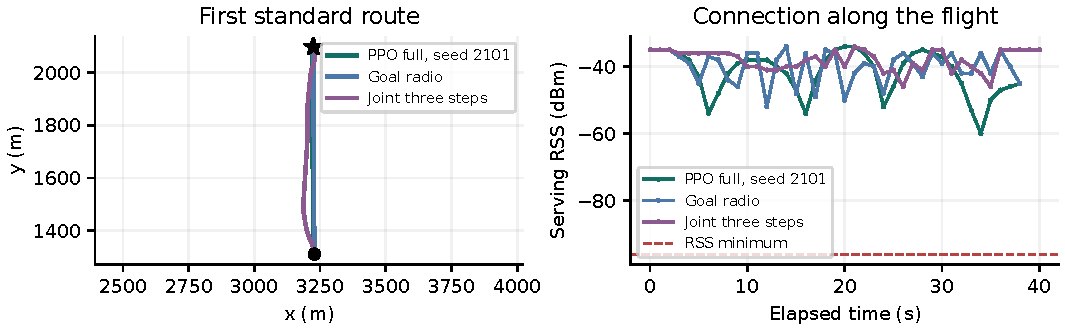
\includegraphics[width=.98\textwidth]{connectivity_example.pdf}
\caption{The first declared standard test route and first full reward training
seed, shown with two model based references. The displayed RSS includes the
initial and terminal sample. This is a fixed example, not a selected typical
route or proof of connectivity between samples.}
\label{fig:example}
\end{figure*}

\section{Validity, Reproducibility and Implications}
The initial test suite contains 34 passing checks covering movement, speed and
acceleration bounds, position and speed arrival conditions, one time success
payment, terminal potential telescoping, finite horizon GAE, mask validity,
likelihood consistency, radio axes and spacing, emergency handovers, identical
dynamics across reward arms, deterministic completion, and seed repeatability.
Reloading the first declared reward only checkpoint reproduces all 200 recorded
standard test episode records exactly. Passing these checks validates important
properties of this code, not equivalence to unavailable source code.

Experiments use Python 3.12, CPU PyTorch 2.4.1, NumPy 2.3.5, and h5py 3.16.0
on a Windows machine with 16 logical processors and approximately 32 GiB RAM.
Study I recorded approximately \TrainingMinutes\ minutes of training and final
validation; Study II recorded 865.68 s. Both exclude map loading and final test
evaluation. The total final training budget is 15,728,640 interactions across
30 policies; pilot budgets are separate.
Checkpoints, all configurations, route splits, training logs, per episode
metrics, source hashes, analysis scripts, and figures are retained locally.
The received map is unchanged and excluded from version control. Independent
reproduction currently requires obtaining that private artifact from its owner;
no public dataset release is claimed.

Several limitations constrain interpretation. First, the shared full state,
continuous actions, and network masks mean the results are not a direct
comparison with the thesis's partially observed discrete controller. Second,
the radio, scheduling, delay, and energy models include declared simplifications;
the full original simulator and exact dataset version remain unverified.
Third, training and testing share one city, one height, one frequency, and one
fixed load pattern. Fourth, five training seeds cannot establish robust tail
behavior. Fifth, the controller is evaluated with deterministic actions and a
fixed training budget, so the measured comparison includes these choices.
Finally, the deterministic reference is already highly effective; the study
does not justify adding a learning controller for this setting on efficiency
grounds alone.

Study II adds 17 behavioral checks for strict RSS and overflow handling,
resource masks, radio costs, the safety filter, action projection, lookahead
isolation, and repeatable PPO parameter updates. All 51 tests pass. Every one
of the 5,600 Study II final evaluations replays exactly; the separate 4,400
flight Study I connectivity audit preserves its original outcomes. The six
Study I and seven Study II frozen source/protocol hashes remain unchanged.
These checks establish implementation consistency, not physical validation.

The frozen Study II estimator contains a generic relative percentage field
for secondary metrics, which is inappropriate for logarithmic SINR values.
Its original statistics are retained. A separate reporting pass sets only
those SINR percentage fields to null and records the original hash; absolute
dB differences, other estimates and every interval are unchanged. This paper
uses absolute SINR differences and reports that correction explicitly.

\subsection{Scientific Interpretation}
The Study I comparison supports repairing the written incentive in the shared
reimplementation. Its observation, dynamics and radio repairs were not
independently ablated, so reward cannot be identified as the sole cause of the
original thesis's behavior. The Study II result concerns a richer controller:
a braking prior, more resource choices, a prospective filter and a wider training
range. Its two arms isolate the communication cost in that architecture; their
results cannot establish a causal reward effect relative to Study I.

The corrected endpoint excludes every sampled RSS or buffer violation from
success. It does not require curved paths, minimum throughput, a packet deadline
or an empty arrival queue. Dense stored RSS coverage makes direct trajectories
plausible. All successful paths meet sampled constraints, while substantial
delay and unsuccessful missions remain possible. The source reciprocal tradeoff
can favor fewer handovers at the expense of delay, as observed in Study II.

Dynamic load, prediction error, switching interruptions, finer temporal
resolution, calibrated energy and independent maps remain untested. Prospective
map access and the motion prior are control components, not learned capabilities.
An application latency or complete delivery requirement would define a new
study, and must not be retroactively imposed on these frozen results.

\balance
\subsection{Availability}
The unified manuscript, source, configurations, raw evaluation records,
analysis code, figures, tests, source snapshots and Markdown research notes are
provided in the project repository:\\
\url{https://github.com/unworthyzeus/UAV_joint_handover_trajectory_optimization}.
The private HDF5 and trained checkpoint binaries remain local and are excluded
from Git. Reproduction therefore requires authorized access to the map and
retraining or separately obtaining checkpoints; this repository is not a
self contained public dataset release. Prior separate manuscript versions are
retained as historical records; this paper is the consolidated scientific report.

\section{Conclusion}
Reward replacement restores destination completion within Study I, whereas
arrival termination alone does not. An audit of those positive results exposes
the gap between reaching the destination and maintaining the required connection.
Study II repairs the sampled RSS and queue endpoint and restores all three
communication objectives. Its full reward lowers weighted cost but increases
delay, and its completion advantage over the arrival arm is uncertain. The
simpler radio selection reference has the highest observed joint completion
among the tested controllers. The result is a documented formulation repair
with useful deterministic evidence and mixed learned results, not a complete
replication of the original thesis or a general PPO superiority claim.

\begin{thebibliography}{00}
\bibitem{thesis} M. Berm\'udez Granados, ``Deep reinforcement learning based joint
handover and trajectory optimization for 5G connected UAV,'' Master's thesis,
Master's Degree in Artificial Intelligence, UPC, UB, and URV, May 2026.
\url{https://upcommons.upc.edu/entities/publication/a8ce08c2-c238-4145-a5ab-5d39b12c6553}.
\bibitem{cherif} N. Cherif, W. Jaafar, H. Yanikomeroglu, and A. Yongacoglu,
``RL-Based Cargo-UAV Trajectory Planning and Cell Association for Minimum
Handoffs, Disconnectivity, and Energy Consumption,'' arXiv:2312.02478, 2023.
\bibitem{hybrid} M. Neunert et al., ``Continuous-Discrete Reinforcement Learning
for Hybrid Control in Robotics,'' in \emph{Proc. Conf. Robot Learning},
PMLR, vol. 100, pp. 735--751, 2020.
\bibitem{masking} S. Huang and S. Onta\~n\'on, ``A Closer Look at Invalid Action
Masking in Policy Gradient Algorithms,'' \emph{Proc. FLAIRS}, vol. 35, 2022,
doi: 10.32473/flairs.v35i.130584.
\bibitem{shaping} A. Y. Ng, D. Harada, and S. Russell, ``Policy invariance under
reward transformations: Theory and application to reward shaping,'' in
\emph{Proc. ICML}, pp. 278--287, 1999.
\bibitem{ppo} J. Schulman, F. Wolski, P. Dhariwal, A. Radford, and O. Klimov,
``Proximal Policy Optimization Algorithms,'' arXiv:1707.06347, 2017.
\bibitem{statistics} R. Agarwal, M. Schwarzer, P. S. Castro, A. C. Courville,
and M. G. Bellemare, ``Deep Reinforcement Learning at the Edge of the
Statistical Precipice,'' in \emph{Adv. Neural Inf. Process. Syst.}, vol. 34, 2021.
\end{thebibliography}
\onecolumn
\appendices
\section{Original TFM and Study I: Complete Model and PPO Comparison}
\label{app:comparison}
The tables compare the written TFM with Study I. Study II retains these
settings except for the explicit changes in Appendix~\ref{app:v2changes}. ``Not
specified'' is an evidence boundary, not an assertion about missing source code.
All shared changes apply even to our legacy arm. Only reward replacement and
training arrival termination are treatment factors. The exact observation layouts appear in Appendix~\ref{app:observations}.
The accompanying note 25 also indexes source definitions and event ordering.

{\centering\footnotesize
\captionof{table}{Environment, objective, and evaluation comparison. Source locators
refer to printed TFM pages. Rows describe shared changes unless marked as factors.}
\label{tab:modelcomparison}
\begin{tabular}{@{}p{.16\textwidth}p{.37\textwidth}p{.42\textwidth}@{}}
\toprule
Item & Original TFM definition & Study I implementation \\
\midrule
Radio environment & Barcelona, 2.1 GHz, 100 m, 133 sites, nominal 1 m grid;
strongest sector RSS~\cite[pp.~6--7, Sec.~3.1, Table~2]{thesis}
& Received map retained; 87 station operator retained. No ray tracing regeneration;
exact source version and sentinel remain unverified. \\
Lookup and geometry & 3D building propagation geometry; lookup and integer
encoding not specified~\cite[pp.~6--7, Sec.~3.1]{thesis}
& Native coordinate spacing, nearest lookup, float radio arithmetic; $-128$
treated as absent path. No collision model. \\
Motion & Scalar speed/selected heading update; five acceleration and eight
heading bins~\cite[p.~9, Eq.~(2); pp.~12, 15]{thesis}
& Inertial velocity, continuous radial/lateral acceleration, norm bound 5 m/s$^2$,
trapezoidal position update, hard speed cap 25 m/s. \\
Time and speed & 1 ms in prose, 0.1 s in table; 2000 timesteps; 100 m/s
penalty threshold~\cite[pp.~14--16, Tables~3--4]{thesis}
& 1 s steps, 200 s deadline. New time discretization and speed constraint. \\
Arrival (factor) & 10 m tolerance, stopping intention, no arrival termination
\cite[p.~9, Sec.~3.2; p.~12, Sec.~5.2; p.~15, Table~3]{thesis}
& Distance $\leq10$ m and speed $\leq2$ m/s. Training termination varied;
every evaluation ends at first safe arrival. \\
Failure handling & Energy termination; boundary/RSS/speed penalties
\cite[p.~12, Sec.~5.2, Eq.~(14)]{thesis}
& Energy exhaustion, boundary crossing, five consecutive RSS outages terminate.
Physical failure precedes arrival; a valid deadline arrival succeeds. \\
Observations & Position, serving BS, RBG, remaining energy, buffer
\cite[p.~12, Sec.~5.2]{thesis}
& 42 scaled features including goal bearing/distance, velocity, time,
consumed energy, prior arrival, phases, serving SINR, candidates, and masks. \\
Network actions & Station and RBG requests, A3 inequality
\cite[p.~9, Eq.~(3); p.~12, Sec.~5.2]{thesis}
& Stay plus top four RSS stations; $>3$ dB advantage and $>-96$ dBm;
five second decisions plus observed outage requests; no time to trigger counters. \\
Resource allocation & Policy requests RBG; availability fallback; random
occupancy of at least half the groups~\cite[pp.~9, 12, 14--15]{thesis}
& RBG is not learned. First free group, exactly six occupied groups per station
in a deterministic pattern; global label phase is not independent load variation. \\
Rate and interference & Bandwidth plus log of SNR; neighboring RSS sum labeled
uplink~\cite[p.~10, Eqs.~(7)--(9)]{thesis}
& Linear downlink cochannel interference, SINR, $B\log_2(1+\mathrm{SINR})$.
Retain 1.44 MHz and $-103.41$ dBm combined noise; change link interpretation. \\
Queue and traffic & Poisson formulation, ratio delay, 160 KB, 4800 bit handover
overhead; conflicting data packet sizes~\cite[pp.~9--10, Eqs.~(4)--(6); pp.~14--15]{thesis}
& Deterministic 200 kbit/s, decimal 1.28 Mbit cap, same handover overhead.
Postservice backlog/rate censored at 200 s; record overflow without terminating. \\
Energy & Mass/efficiency/lift-to-drag expression; capacity labeled 1000 kW
\cite[p.~10, Eq.~(10); p.~15, Table~3]{thesis}
& Consumed energy integral of $100+0.4v^2$ W; 100 kJ budget. New uncalibrated
proxy, not a conversion of original capacity. \\
Reward (factor) & Positive reciprocals, binary $+12$ progress, penalties
\cite[p.~12, Eqs.~(13)--(14); p.~15, Table~3]{thesis}
& Legacy structure uses new common physical inputs and no soft speed penalty.
Replacement adds first arrival/terminal failure payments, time cost, bounded
radio costs, and terminal corrected potential shaping. \\
Deterministic reference & Constant speed, closest discrete heading, viability
counters~\cite[pp.~13--14, Sec.~5.4]{thesis}
& Continuous desired velocity tracking with braking; strongest admissible
station and shared masks. A new reference, not a reproduction of that greedy policy. \\
Splits and comparison & PPO/greedy and weight comparisons; separate validation
and test sets not specified~\cite[pp.~15--16, Secs.~6.2--6.3]{thesis}
& 4096 training, 64 validation, 200 standard test, 200 longer test routes;
five seeds per treatment, frozen budget. Same map, not a geographic holdout. \\
Reported outcomes & SNR, outage, interference, remaining energy, handovers,
example paths~\cite[pp.~16--20, Sec.~7]{thesis}
& Mission and recorded feasible success first; secondary metrics conditional
on success; every seed, paired bootstrap and failure counts retained. \\
\bottomrule
\end{tabular}
}

For completeness, our reset sets velocity, queue, consumed energy, counters,
and prior arrival to zero, associates with the strongest station, and allocates
its first free group. Each step applies the requested admissible handover before
motion, evaluates radio after motion, updates queue and energy, checks failure
and arrival, and then computes reward. The TFM does not fully specify this
event ordering~\cite[pp.~9--12, Secs.~3.2--5.2]{thesis}.
The direct energy and packet overflow reward terms removed during the original
development~\cite[pp.~20--21, Sec.~7.3]{thesis} are not treated as part of its
final reward. We also do not claim to have reproduced its mass or efficiency
model, random traffic, counter based handovers, or learned resource allocation.

\clearpage
{\centering\footnotesize
\captionof{table}{PPO comparison. The first eleven rows cover every parameter in the
original Table 4~\cite[p.~16]{thesis}. Further implementation details are not
fully specified in its Secs. 5.3 and 6.2~\cite[p.~13; pp.~15--16]{thesis}.}
\label{tab:ppocomparison}
\begin{tabular}{@{}p{.25\textwidth}p{.20\textwidth}p{.50\textwidth}@{}}
\toprule
Parameter & Original TFM & Study I implementation \\
\midrule
Episodes & 300 & Fixed interactions, variable number of episodes \\
Episode timesteps & 2000 & 200, with explicit early terminals \\
Rollout steps per environment & 8 & 128 \\
Learning rate & $3\cdot10^{-5}$ & $3\cdot10^{-4}$, constant \\
Batch size & 32 & 512 \\
Discount & 0.99 & 0.99, retained \\
GAE lambda & 0.95 & 0.95, retained \\
Policy clip & 0.2 & 0.2, retained \\
Value coefficient & 0.5 & 0.5 applied to half MSE; total coefficient 0.25 MSE \\
Entropy coefficient & 0.01 & 0.005 \\
Target KL & 0.03 & No threshold; log diagnostic KL only \\
\midrule
Implementation & Stable Baselines & Native PyTorch hybrid PPO \\
Parallel lanes and update epochs & Not specified & 64 lanes; 8192 samples per rollout; four epochs \\
Interaction budget & Episodes/timesteps listed & 524,288 per policy, 64 rollout updates \\
Networks & Not specified & Separate actor/critic, each two 64 unit tanh layers \\
Policy heads & Discrete action vector listed & 2D Gaussian plus masked five choice categorical \\
Initialization and variance & Not specified & Orthogonal weights; log standard deviation initialized $-0.5$,
clamped to $[-2.3,0.5]$ \\
Optimizer and gradient cap & Adam in pseudocode & Adam, epsilon $10^{-5}$, gradient norm cap 0.5 \\
Likelihood and entropy details & Not specified & Latent Gaussian likelihood after stored action sampling;
sum latent Gaussian and categorical entropy \\
Reward and advantage scaling & Not specified & Running discounted return variance; no reward centering;
reward clip $[-10,10]$; minibatch advantage normalization \\
Critic and bootstrap details & Not fully specified & Unclipped half MSE; bootstrap only across nonterminal
rollout ends, not across mission/deadline terminals \\
Evaluation and checkpoint rule & Not specified & Gaussian mean and categorical mode; final checkpoint only;
common raw evaluation reward for every treatment \\
\bottomrule
\end{tabular}
\vspace{1.5em}
}

\bigskip
\section{Every Executed Change from Study I to Study II}
\label{app:v2changes}
This inventory compares final frozen implementations, including choices that
were retained. Original locators refer to the written TFM, not recovered code.
The inherited serialized field \texttt{max\_consecutive\_outage: 5} is unused by
Study II: its executed step fails on the first violation. Remaining queue at
arrival and instantaneous switching are retained limitations.

{\footnotesize\setlength{\tabcolsep}{3pt}
\begin{longtable}{@{}p{0.13\textwidth}p{0.23\textwidth}p{0.31\textwidth}p{0.28\textwidth}@{}}
\caption{Final Study II differences and original source relationships.}\label{tab:v2changes}\\
\toprule Item & v1 executed behavior & Final v2 executed behavior & Original source relationship\\\midrule
\endfirsthead
\multicolumn{4}{l}{\textit{Continued from previous page}}\\\toprule
Item & v1 executed behavior & Final v2 executed behavior & Original source relationship\\\midrule
\endhead
\bottomrule\endfoot
Minimum RSS & RSS $\leq$ -96 dBm counts as outage. & RSS < -96 dBm counts as violation; equality is allowed. & Follow C2's $\geq$ inequality \cite[p. 11, Eq. (12)]{thesis} and the numeric minimum \cite[p. 15, Table 3]{thesis}.\\
Initial RSS & Strongest station selected at reset; no separate persistent initial violation flag. & Check the initial serving RSS and preserve any violation until failure. & Include the initial modeled sample in C2 \cite[p. 11]{thesis}.\\
Failure rule & Five consecutive sampled outages terminate a flight. & Any single sampled RSS violation terminates a failed joint mission. & Enforce the written C2 at modeled samples \cite[p. 11]{thesis}, rather than reproduce the source's soft reward penalty \cite[p. 12, Eq. (14)]{thesis}.\\
Buffer overflow & Count lost bits, clip queue, continue flight; disqualify only the subsequent feasible label. & Any overflow ends failure; clipping cannot erase it. & Enforce C4 at the sampled queue update \cite[p. 11, Eq. (12)]{thesis}. Source removal of a direct dump penalty is described on pp. 20--21, Sec. 7.3.\\
Joint success & Arrival is primary; recorded feasibility permits up to 5\% RSS outage and zero drops. & Arrival plus no prior sampled RSS violation, no overflow, and no physical failure. No additional permissive feasibility label. & Combine source communication constraints \cite[p. 11]{thesis} with explicit destination completion.\\
Event precedence & Some physical failures override arrival; overflow does not. & RSS, overflow, boundary and energy failure override simultaneous arrival. & New explicit ordering; original source ordering is unspecified \cite[p. 12, Sec. 5.2]{thesis}.\\
Outstanding queue at arrival & Allowed. & Still allowed and reported. & The source does not specify an empty queue arrival test \cite[pp. 9--12, Secs. 3.2--5.2]{thesis}. We do not claim all generated data has been delivered.\\
Delay cost & 0.05 * min(D, 1) inside fixed reward. & 0.35 * 10D / (1 + 10D) in full arm. No flat reward plateau at one second. & One minus original reciprocal utility \cite[p. 12, Eq. (13)]{thesis} with equal configuration values \cite[p. 15, Table 3]{thesis}. Smooth saturation remains.\\
Interference cost & Absent from fixed reward, although measured. & Restore 0.30 * 100000I / (1 + 100000I). & Same reciprocal utility scales and weights \cite[pp. 12, 15]{thesis}. I remains our downlink proxy.\\
Handover cost & 0.05 * H. & 0.35 * 100H / (1 + 100H). & Restore normalized source utility \cite[p. 12, Eq. (13); p. 15, Table 3]{thesis}.\\
Positive per step radio utility & Present in reimplemented legacy reward, removed in v1 fixed reward. & Subtract communication cost, so simply staying active does not earn that utility bonus. & Changes the positive reciprocal reward structure \cite[p. 12, Eqs. (13)--(14)]{thesis} while preserving the three normalized tradeoff components.\\
Learning comparison & Four reward/termination arms; direct acceleration learning. & Two arms: arrival base only versus arrival base minus all three radio costs. Both use strict failure, termination and the same new controller architecture. & A new controlled comparison; neither arm is the source's trained policy.\\
Network decision timing & Every five seconds, with observed outage exception. & Every modeled second. & Source describes choices each environment step \cite[pp. 9, 12, Secs. 3.3.1, 5.2]{thesis}; a five second interval was our prior assumption.\\
Network action & Stay plus four strongest candidate stations: five categorical choices. & Stay plus five candidate station slots by 12 groups: 61 choices. & Restores resource choice from the source's BS/RBG action \cite[p. 12, Sec. 5.2]{thesis}.\\
Station candidate selection & Serving plus strongest four, stable RSS ordering. & Retained. Duplicate serving station slots are masked. & Restricted candidate interface is ours; source lists full BS/RBG choices \cite[p. 12]{thesis}.\\
A3 condition & Candidate RSS > serving RSS + 3 dB. & Retained; prospective filter cannot bypass it. & Follow the inequality, not the reversed nearby prose \cite[p. 9, Eq. (3); p. 15, Table 3]{thesis}.\\
Resource allocation & Deterministic first free RBG at reset and handover. & That initialization remains; the controller can choose any currently free RBG, including within the same station. & Source allows RBG requests with fallback \cite[p. 9, Sec. 3.3.1]{thesis}. The exact masking implementation is ours.\\
Repeating a resource choice & No learned resource choice. & Current serving station/group pair remains a valid pair action; explicit stay also remains. & Avoid a new artificial alternating action mask; this is an implementation decision.\\
Resource change count & Not independently reported. & Count every station/group change, including same station RBG changes. & Diagnostic addition. Same station resource changes are not counted as handovers.\\
Switching interruption & Not modeled. & Still not modeled; no extra RBG switching cost. & Source does not provide a calibrated interruption duration \cite[p. 9, Sec. 3.3.1; p. 15, Table 3]{thesis}. This remains a limitation, not a verified original behavior.\\
Continuous action & Two direct radial/lateral acceleration commands. & Projected reference command plus two bounded learned residuals of scale 0.5, followed by physical projection. & New controller prior; differs from original discrete acceleration and heading \cite[p. 12, Sec. 5.2; p. 15, Table 3]{thesis}.\\
Safety filter & None. & Predict the next sample; repair unsafe network choice if possible, otherwise try local motion/network alternatives; still fail if unresolved. & New model based constraint handling component; original source describes reward penalties \cite[p. 12, Eq. (14)]{thesis}.\\
Prospective radio access & Learned policy observes current candidates. & PPO still observes current options. Its shared filter and model based references query the known map at predicted positions. & New information/control architecture, not reproduced source logic.\\
Observation & 42 features. & 156 features, detailed below. & Original source has six listed state elements \cite[p. 12, Sec. 5.2]{thesis}. Both are reimplementations with repaired state.\\
PPO network head & Five categorical logits. & 61 categorical logits; continuous and value heads retained. & Original architecture details are not sufficiently specified \cite[p. 13, Sec. 5.3]{thesis}.\\
Training route lengths & 200--1000 m. & 200--1800 m; longer tests lie within this range. & New study design; original route distribution and independent splits are not documented \cite[pp. 15--16, Secs. 6.2--6.3]{thesis}.\\
Final route identities & Seeds 42012 and 42013. & Fresh seeds 52012 and 52013. Exact pairs are disjoint from v1 and other v2 splits. & Our explicit split protocol; same map remains shared.\\
Training seeds & 1101--1105. & 2101--2105. & New repeated experiment; original seed list is unspecified \cite[pp. 15--16]{thesis}.\\
Final budget & 524,288 interactions each; 20 policies. & Same interactions per policy; 10 policies. & Our PPO budget remains different from 300 episodes and 2,000 maximum steps in the source \cite[p. 16, Table 4]{thesis}.\\
Deterministic references & Destination braking and strongest admissible RSS. & Four nominal control laws with the same filter: Goal RSS, Goal radio, one step joint search, and three step joint search. & New references, not a recreation of the thesis's discrete constant velocity greedy controller \cite[pp. 13--14, Sec. 5.4]{thesis}.\\
Secondary comparison & Success conditioned summaries and selected matched comparisons. & Explicit intersections of successful route/seed pairs for radio comparisons, with counts and crossed bootstrap intervals. & Source does not report a matching conditional joint success protocol \cite[pp. 16--20, Sec. 7]{thesis}.\\
\end{longtable}}
\clearpage
\section{Exact Observation and Numerical Interfaces}
\label{app:observations}
All indices are zero based. Study I has 42 features; Study II has 156. Both
replace the original listed position, station, resource, energy and queue vector
\cite[p.~12, Sec.~5.2]{thesis}. Scales are fixed; no fitted observation normalizer
is used. Study II removes the prior arrival flag, consecutive outage count and
five second phase because arrival and RSS failure now terminate immediately.

{\footnotesize\setlength{\tabcolsep}{3pt}
\begin{longtable}{@{}p{0.13\textwidth}p{0.82\textwidth}@{}}
\caption{Study I observation indices and scales.}\label{tab:obs1}\\
\toprule Indices & Features and scaling\\\midrule
\endfirsthead
\multicolumn{2}{l}{\textit{Continued from previous page}}\\\toprule
Indices & Features and scaling\\\midrule
\endhead
\bottomrule\endfoot
0--1 & Position divided by (5000, 3500)\\
2--3 & Unit vector toward goal; (1, 0) fallback at effectively zero distance\\
4 & Goal distance / 1000 m\\
5--6 & Velocity projected onto radial and lateral directions / 25 m/s\\
7 & Speed / 25 m/s\\
8 & Elapsed steps / 200; determines remaining time\\
9 & Queue bits / 1,280,000\\
10 & Consumed energy / 100,000 J, rather than remaining energy\\
11 & Whether first safe arrival already occurred\\
12--13 & Resource label phase / 11 and allocated RBG / 11\\
14 & (step mod 5) / 5\\
15 & Serving SINR in dB / 30\\
16 & Consecutive outage samples / 5\\
17--21 & Five candidate RSS values, each transformed as (RSS + 70) / 60\\
22--31 & Candidate station x/y offsets from UAV, both divided by 5000 m\\
32--36 & Candidate indices within selected operator / 86, not global station IDs or one hot vectors\\
37--41 & Five Boolean admissibility flags represented as float features\\
\end{longtable}}

{\footnotesize\setlength{\tabcolsep}{3pt}
\begin{longtable}{@{}p{0.13\textwidth}p{0.82\textwidth}@{}}
\caption{Study II observation indices and scales.}\label{tab:obs2}\\
\toprule Zero based indices & Definition\\\midrule
\endfirsthead
\multicolumn{2}{l}{\textit{Continued from previous page}}\\\toprule
Zero based indices & Definition\\\midrule
\endhead
\bottomrule\endfoot
0--1 & Position / map dimensions\\
2--3 & Destination direction unit vector\\
4 & Destination distance / 1,000 m\\
5--6 & Radial and lateral velocity / 25 m/s\\
7 & Speed / 25 m/s\\
8 & Elapsed decision count / 200\\
9 & Queue / 1,280,000 bits\\
10 & Consumed energy / 100,000 J\\
11--12 & Background phase / 11 and serving RBG / 11\\
13 & Serving SINR in dB / 30\\
14--18 & Candidate RSS, transformed as (RSS + 70) / 60\\
19--28 & Candidate station x/y offsets / 5,000 m\\
29--33 & Candidate station index / 86\\
34--94 & log(1 + option\_capacity / 200000) for all 61 network choices\\
95--155 & Corresponding Boolean action masks as float features\\
\end{longtable}}

For station index $k$, episode label phase $z$, and group $g$, background
occupancy is $\ind[(g-(7k+z))\bmod12<6]$. The reset allocator chooses
$(7k+z+6)\bmod12$. Phase $z$ rotates labels globally; it does not yield independent
load fields. Each vector lane is an independent single UAV mission. The source
describes random occupancy of at least half the groups
\cite[p.~14, Sec.~6.1; p.~15, Table~3]{thesis}.

Both studies use postservice backlog divided by service rate, censored at 200 s,
as delay. A zero service rate is handled numerically rather than interpreted
as a measured packet latency. The shared queue generates offered bits and any
handover overhead, serves the queue at the modeled capacity, records excess
above its capacity and clips for storage. Study II additionally fails on that
excess. Stored $-128$ RSS supplies zero power; SINR reporting has a $10^{-15}$
logarithm floor. These declarations complement the original queue and rate
expressions~\cite[pp.~9--10, Eqs.~(4)--(9)]{thesis}.

Study I evaluates every checkpoint using the common fixed raw reward by default;
its stored return is an undiscounted evaluation sum, not its PPO normalized
training return. Success and physical metrics define the reported comparisons.
In continuing training, first arrival pays its bonus once; a later failure
cannot pay the prearrival failure penalty. Study II always terminates on joint
success or first failure and scores the proposed residual/network action before
environment projection and safety filtering. Neither study has a separate soft
speed penalty, since the shared dynamics impose the cap.

\clearpage
\section{Development Evidence and Artifact Map}
\label{app:development}
Development results below use only 64 standard and 32 longer validation routes.
Each row uses one seed per arm and is exploratory; it does not estimate final
seed uncertainty. All six Study II pilot checkpoints and source snapshots are
retained locally. Study I retains six pilots with seeds 41 and 42, including
the validation curve in Fig.~\ref{fig:pilot}. No pilot checkpoint initializes a
final policy.

{\footnotesize\setlength{\tabcolsep}{3pt}
\begin{longtable}{@{}p{0.34\textwidth}p{0.21\textwidth}p{0.2\textwidth}p{0.2\textwidth}@{}}
\caption{Study II pilot development; percentages are standard / longer joint success.}\label{tab:development}\\
\toprule Design & Pilot seed and budget per arm & Arrival arm standard / longer joint success & Full arm standard / longer joint success\\\midrule
\endfirsthead
\multicolumn{4}{l}{\textit{Continued from previous page}}\\\toprule
Design & Pilot seed and budget per arm & Arrival arm standard / longer joint success & Full arm standard / longer joint success\\\midrule
\endhead
\bottomrule\endfoot
Direct motion, no filter, short training lengths & 51; 524,288 & 89.1\% / 59.4\% & 92.2\% / 34.4\%\\
Direct motion, safety filter, short training lengths & 52; 1,048,576 & 92.2\% / 78.1\% & 98.4\% / 75.0\%\\
Residual motion, safety filter, 200--1800 m training lengths & 53; 524,288 & 96.9\% / 84.4\% & 98.4\% / 87.5\%\\
\end{longtable}}

The first strict nominal RSS controller completed 95.3\% / 71.9\% of validation
routes; prospective radio selection completed 96.9\% / 90.6\%. A local joint
search initially completed 95.3\% / 81.3\% and sometimes preferred stationary
low cost states. A preference for immediate progress, with the shared filter,
raised its observed validation completion to 98.4\% / 87.5\%. The filtered
radio reference reached 96.9\% / 93.8\%. A three step lookahead design initially
postponed movement at each replan, reaching 70.3\% / 53.1\%; applying progress
preference to the first predicted step yielded 93.8\% / 87.5\%, still with three
standard timeouts. These development failures are retained, not hidden by the
final controller selection.

In the second pilot design, the current station/group pair remained legal in
addition to explicit stay, eliminating an artificial alternating resource mask.
The third design introduced the residual braking prior and 200--1800 m training
range. No communication threshold was relaxed. The full final pilot already
showed fewer handovers and higher delay, motivating explicit component reporting
in the frozen comparison. These simultaneous development changes do not identify
individual causal contributions.

The following artifact families give a reproducible route from source data to
this paper. They are paths relative to the repository root; private binaries
are retained locally. Markdown notes 17--27 cover Study I and its audit, notes
28--32 cover Study II, and note 33 records this consolidation and publication.

{\footnotesize\setlength{\tabcolsep}{3pt}
\begin{longtable}{@{}p{0.16\textwidth}p{0.79\textwidth}@{}}
\caption{Artifacts and reproducibility boundaries.}\label{tab:artifacts}\\
\toprule Artifact & Location / purpose\\\midrule
\endfirsthead
\multicolumn{2}{l}{\textit{Continued from previous page}}\\\toprule
Artifact & Location / purpose\\\midrule
\endhead
\bottomrule\endfoot
Original map & dataset/Barcelona\_dataset\_January.h5; unchanged private HDF5, excluded from Git; SHA256 is stored in both freeze manifests.\\
Study I freeze & configs/frozen\_comparison\_v1.json; six exact source/protocol hashes.\\
Study II freeze & configs/frozen\_connectivity\_v2.json; seven exact source/protocol hashes.\\
Routes & configs/controlled\_scenarios.json and configs/connectivity\_scenarios\_v2.json; saved coordinate pairs, phases and seeds.\\
Outcomes & results/controlled\_experiment/confirmatory\_v1/ and results/connectivity\_experiment/confirmatory\_v2/; final evaluation records, training logs and source snapshots.\\
Statistics & Corresponding analysis\_v1/ and analysis\_v2/ directories; raw estimators, paired intervals, generated figures and table inputs. Study II report\_statistics.json documents the SINR reporting correction.\\
Replay & results/controlled\_experiment/connectivity\_audit\_v1/ and results/connectivity\_experiment/replay\_v2/; 4,400 audit and 5,600 final exact replays respectively.\\
Paper & paper/unified.tex and paper/unified\_appendices.tex; shared generated tables and figures; final consolidated IEEE format draft.\\
\end{longtable}}

\end{document}
